\section{GraphBLAS objects}
\label{sec:GrBObjects}

The GraphBLAS C API is built on objects exposed to 
the C programmer as opaque data types. These objects include
\begin{itemize}
\item \emph{Collections}: vectors and matrices.
\item \emph{Algebraic objects}: unary and binary operators, monoids, and semirings.
\item \emph{Control objects}: descriptors and masks (both one- and two-dimensional).
\end{itemize}

Functions that manipulate GraphBLAS objects
are referred to as {\it methods}.  These methods fully define the 
interface to create or destroy GraphBLAS objects, modify their 
contents, and copy the contents of opaque objects into non-opaque or \emph{transparent} 
objects, the contents of which are under direct observation and control of the programmer

\subsection{Collections}
\label{Sec:Collections}

The state of a GraphBLAS application is largely captured by collections of values, 
namely vectors and matrices.  The GraphBLAS collections 
are opaque objects only accessible through the methods in the GraphBLAS C API.
The use of opaque data types gives the implementation the flexibility needed to 
aggressively optimize for different system architectures.

A GraphBLAS vector $\vector{v} = \langle D, N, \{ (i,v_i) \} \rangle$ is defined by:
\begin{itemize}
\item The domain $D$, which is the data type for the elements of the vector.
\item The size $N>0$.
\item A set of tuples $(i,v_i)$ where $0 \leq
i < N$ and $v_i \in D$. 
\end{itemize}
A particular value of $i$ can only appear at
most once in $\vector{v}$. We define $\mathbf{nelem}(\vector{v}) = N$ and
$\mathbf{L}(\vector{v}) = \{ (i,v_i) \}$. The set $\mathbf{L}(\vector{v})$ is
called the \emph{content} of vector $\vector{v}$. 
%%%%
% TGM:  Any concepts we don't use in the paper should not be introduced, 
% hence why these are commented out
%%%%
%We also define the set:
%$$
%\vector{ind(\vector{v})} = \{ i : (i,v_i) \in \mathbf{L}(\vector{v}) \}
%$$
%(called the \emph{structure} of $\vector{v}$), and $\mathbf{D}(\vector{v})
%= D$. 
For a vector $\vector{v}$, $\vector{v}(i)$ is a reference to $v_i$
if $(i,v_i) \in \mathbf{L}(\vector{v})$ and is undefined otherwise. 

A GraphBLAS matrix  $\matrix{A} = \langle D, M, N, \{ (i,j,A_{ij}) \} \rangle$ is
defined by:
\begin{itemize}
\item The domain $D$, which is the data type for the elements of the matrix.
\item The number of rows $M>0$ and columns $N>0$.
\item A set of tuples $\mathbf{L}(\matrix{A}) = (i,j,A_{ij})$ where $0 \leq i < M$, $0 \leq
j < N$, and $A_{ij} \in D$. 
\end{itemize}
A particular pair of values $i,j$ can only
appear at most once in $\matrix{A}$. 
The set $\mathbf{L}(\matrix{A})$ is called the
\emph{content} of matrix $\matrix{A}$.  
We also define $\mathbf{nrows}(\matrix{A}) = M$ and 
$\mathbf{ncols}(\matrix{A}) = N$.
%%%%%
% TGM: if we don't use a notation in this paper, then I don't want to introduce it
%%%%%
%We define $\mathbf{ncols}(\matrix{A})
%= N$,  $\mathbf{nrows}(\matrix{A}) = M$ and $\mathbf{L}(\matrix{A}) =
%\{ (i,j,A_{ij}) \}$.  
%We also define the sets:
%$$
%\vector{indrow(\matrix{A})} = \{ i : \exists (i,j,A_{ij}) \in \matrix{A} \}
%$$
%$$
%\vector{indcol(\matrix{A})} = \{ j : \exists(i,j,A_{ij}) \in \matrix{A} \}
%$$  
%These are the sets of nonempty
%rows and columns of $\matrix{A}$, respectively.)  The \emph{structure}
%of matrix $\matrix{A}$ is the set 
%$$
%\mathbf{ind}(\matrix{A}) = \{ (i,j) :(i,j,A_{ij}) \in \mathbf{L}(\matrix{A}) \}
%$$
%and $\mathbf{D}(\matrix{A}) = D$.
For a matrix $\matrix{A}$, $\matrix{A}(i,j)$ is a reference to $A_{ij}$
if $(i,j,A_{ij}) \in \mathbf{L}(\matrix{A})$ and is undefined otherwise.  

The fact that matrix and vector elements can be undefined is an essential difference between GraphBLAS
and more traditional sparse matrix packages for which elements that are not
explicitly stored are assumed to have the numerical value $0$.   We leave these
elements as undefined to avoid the complexity of interpreting these implied
values differently as the operation semiring changes.

If $\matrix{A}$ is a matrix and $0 \leq j < N$, then 
$$ \matrix{A}(:,j)= \langle D, M, \{(i,A_{ij}) : (i,j,A_{ij}) \in \mathbf{L}(\matrix{A})\} \rangle
$$
is a vector called the $j$-th \emph{column}
of $\matrix{A}$. Correspondingly, if $\matrix{A}$ is a matrix and
$0 \leq i < M$, then 
$$
\matrix{A}(i,:) = \langle D, N, \{(j,A_{ij}) :(i,j,A_{ij}) \in \mathbf{L}(\matrix{A}) \} \rangle
$$ 
is a vector called
the $i$-th \emph{row} of $\matrix{A}$.

We define the transpose of a matrix in the traditional manner where
row and column indices are swapped.   Consider a matrix 
$
\matrix{A} = \langle D, M, N, \{ (i,j,A_{ij}) \} \rangle,
$
the \emph{transpose} of $\matrix{A}$ is the matrix 
$$
\matrix{A}^T = \langle D, N, M, \{(j,i,A_{ij}) : (i,j,A_{ij}) \in \mathbf{L}(\matrix{A}) \} \rangle.
$$

\subsection{Algebraic objects}
\label{Sec:AlgebraicObjects}

The GraphBLAS differs from traditional sparse linear algebra APIs in that the
algebra associated with the data can be varied to match the needs
of an application.  Pragmatically, this means the API was designed to
provide a great deal of flexibility in the domains of the elements in the GraphBLAS
collections and the operations defined between these elements.

We start with  basic binary and unary operators.  
A GraphBLAS \emph{binary operator} is defined as:
$$
F_b = \langle D_1, D_2, D_3, \odot \rangle.
$$
It has three domains, $D_1$, $D_2$, $D_3$, and an operation
$$
\odot: D_1 \times D_2 \rightarrow D_3.
$$
%For a given GraphBLAS operators
%$$
%F_b=\langle D_1, D_2, D_3,\odot \rangle
%$$ we define $\mathbf{D}_1(F_b) = D_1$,
%$\mathbf{D}_2(F_b) = D_2$, $\mathbf{D}_3(F_b) = D_3$, and $\mathbf{\bigodot}(F_b)
%= \odot$.  Note that $\odot$ could be used in place of either $\oplus$ or $\otimes$.
A GraphBLAS \emph{unary operators} is defined as:
$$
F_u = \langle D_1, D_2, f\rangle.
$$
It has two domains, $D_1$, $D_2$, and an operation
$f: D_1 \rightarrow D_2$.  
%For a given GraphBLAS operators
%$$
%F_u=\langle D_1, D_2, f \rangle
%$$ we define $\mathbf{D}_1(F_u) = D_1$,
%$\mathbf{D}_2(F_u) = D_2$, and $\mathbf{f}(F)
%= f$.
%

GraphBLAS makes use of two fundamental algebraic structures: monoids
and semirings.   
A GraphBLAS  \emph{monoid} 
$$
M =\langle D_1,\odot,\mathbf{0} \rangle
$$ 
is defined by a single domain $D_1$, an 
\emph{associative}\footnote{It is expected that implementations 
will utilize IEEE-754 floating point arithmetic which is not 
strictly associative.} 
operation $\odot: D_1 \times D_1 \rightarrow D_1$,
and an identity element $\mathbf{0} \in D_1$.  
%For a given GraphBLAS monoid
%$$
%M=\langle D_1,\odot,0 \rangle
%$$ 
%we define $\mathbf{D}_1(M) = D_1$, $\mathbf{\bigodot}(M) =
%\odot$ and $\mathbf{0}(M) = 0$.  
Let
$
F = \langle D_1,D_1,D_1,\odot \rangle
$ 
be a GraphBLAS binary operator and let
$\mathbf{0}$ be the identity for $\odot$. Then 
$$
M = \langle F,\mathbf{0} \rangle = \langle
D_1,\odot,\mathbf{0} \rangle
$$ 
is the associated GraphBLAS monoid.

The algebraic structure at the core of the GraphBLAS is the semiring.  
A GraphBLAS \emph{semiring} 
$$
S=\langle D_1,D_2,D_3,\oplus,\otimes,\mathbf{0} \rangle
$$ 
is defined by
three domains $D_1$, $D_2$ and $D_3$, an \emph{associative}
additive operation 
$$
\oplus : D_3 \times D_3 \rightarrow D_3
$$
a multiplicative operation 
$$\otimes : D_1 \times D_2 \rightarrow
D_3
$$
and an element $\mathbf{0} \in D_3$, which is the identity for $\oplus$.
%For a given GraphBLAS semiring 
%$$
%S=\langle D_1,
%D_2, D_3,\oplus,\otimes,0 \rangle
%$$ 
%we define $\mathbf{D}_1(S) = D_1$,
%$\mathbf{D}_2(S) = D_2$, $\mathbf{D}_3(S) = D_3$, $\mathbf{\bigoplus}(S) =
%\oplus$, $\mathbf{\bigotimes}(S) = \otimes$, and $\zero(S) = 0$. 

Let $F = \langle D_1,D_2,D_3,\otimes \rangle$ be a GraphBLAS binary operator
and let $M = \langle D_3,\oplus,\mathbf{0} \rangle$ be a GraphBLAS monoid,
then 
$$
S= \langle M,F \rangle = \langle D_1,D_2,D_3,\oplus,\otimes,\mathbf{0} \rangle
$$
is a GraphBLAS semiring.

Correspondingly, for a GraphBLAS semiring 
$S = \langle D_1,D_2,D_3,\oplus,\otimes,\mathbf{0} \rangle$
there is always an associated monoid 
$M = \langle D_3,\oplus,\mathbf{0} \rangle$ and
an associated binary operator $F = \langle D_1,D_2,D_3,\otimes \rangle$.

A UML diagram of the conceptual hierarchy of Algebraic objects in GraphBLAS
algebra (binary operators, monoids and semirings) is shown in 
Figure~\ref{Fig:AlgebraHierarchy}.

\begin{figure}[htb]
    \hrule
    \begin{center}
        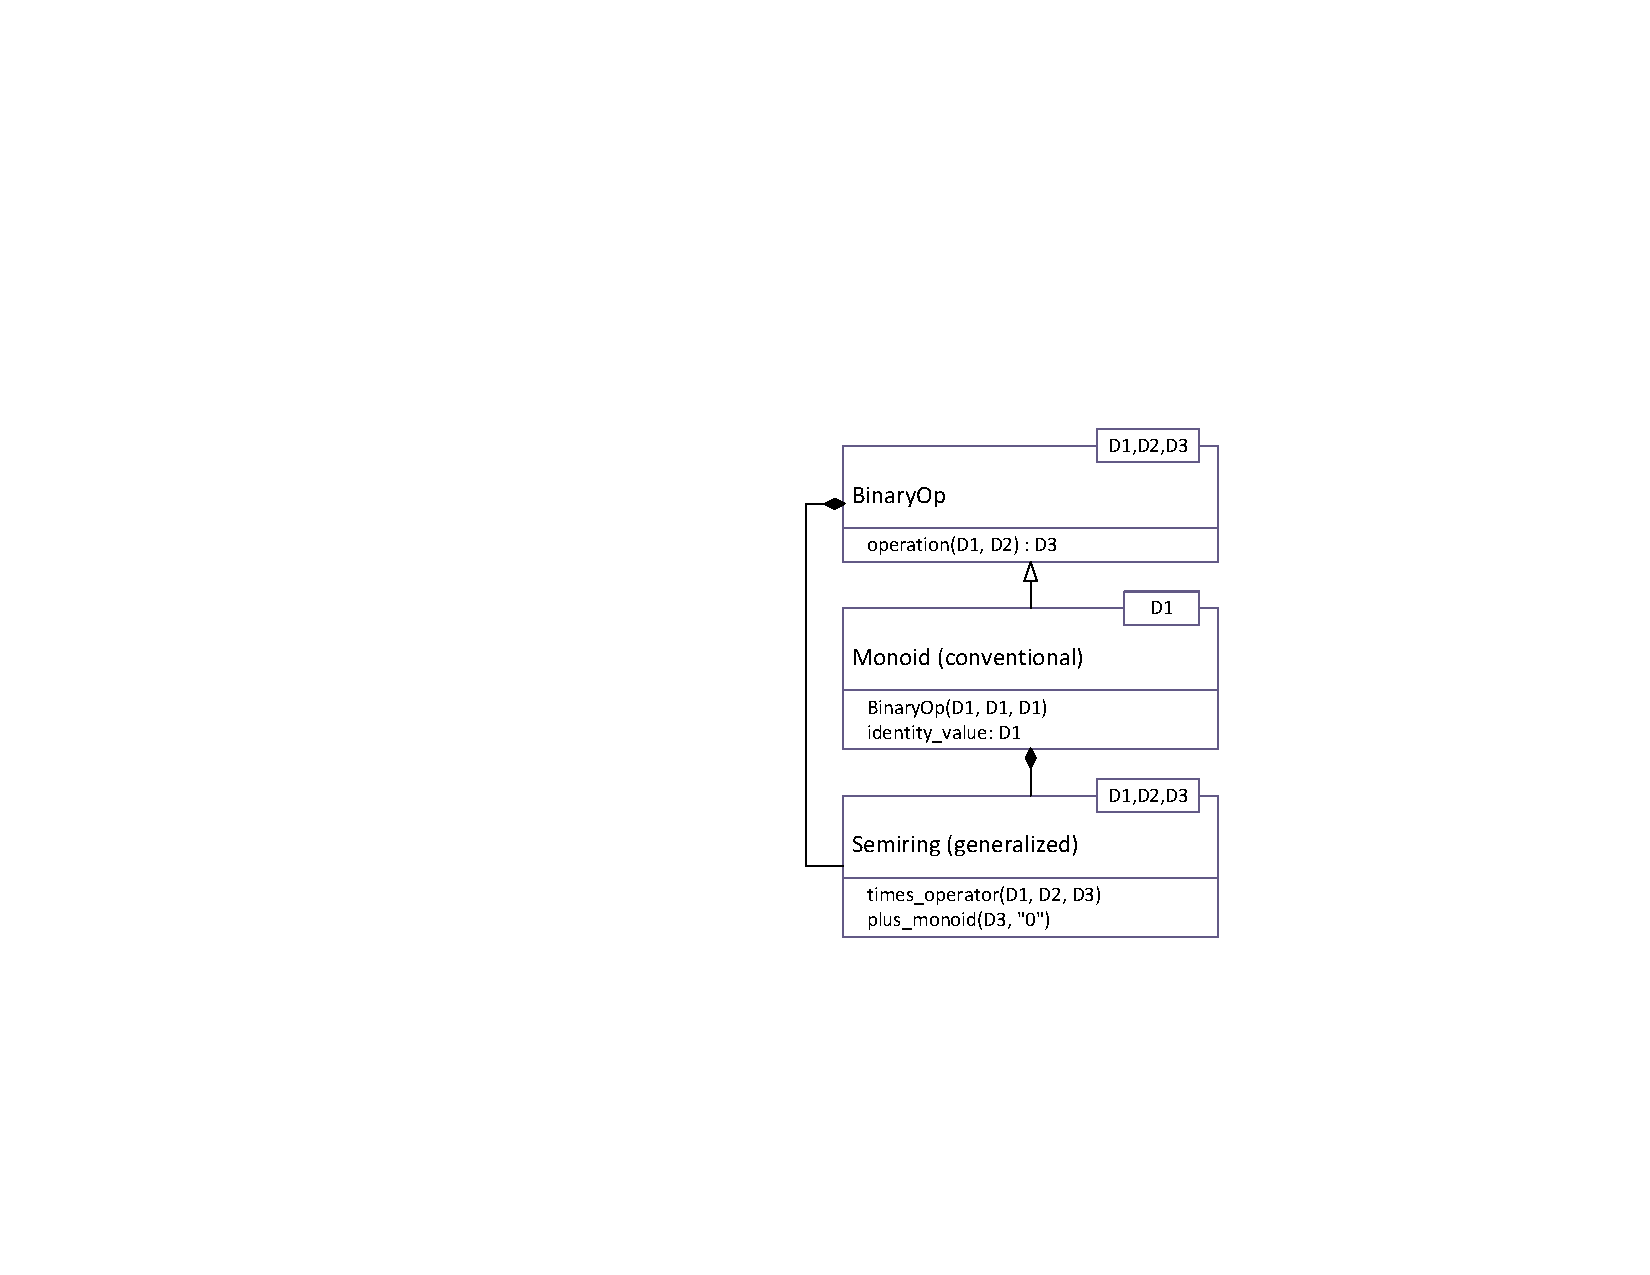
\includegraphics[width=1.0\linewidth,trim=3in 2in 0.5in 2in]{Algebra_Hierarchy_v2.pdf}
    \end{center}
    \caption{Hierarchy of algebraic object classes in GraphBLAS. GraphBLAS semirings consist of a conventional monoid with one domain for the addition function, and a binary operator with three domains for the multiplication function.}
    \label{Fig:AlgebraHierarchy}
    \hrule
\end{figure}


\subsection{Control objects}
\label{Sec:ControlObjects}

The GraphBLAS C API specification defines two opaque objects that 
modify the semantics of GraphBLAS methods; \emph{masks} and 
\emph{descriptors}.  

A mask can be either a one- or a two-dimensional construct.  One- and
two-dimensional masks, described more formally below, are similar to
vectors and matrices, respectively, except that they have structure
(indices) but no values. Masks are used to control which values from 
a operation are written to the output object.

A one-dimensional mask $\vector{m} = \langle N, \{ i \} \rangle$ is
defined by its number of elements $N>0$ and a set $\mathbf{L}(\vector{m})$
of indices $\{ i \}$ where $0 \leq i < N$.  A particular value of $i$ can
only appear at most once in $\vector{m}$. We define $\mathbf{nelem}(\vector{m})
= N$.  
We define the \emph{structure} of a one dimensional mask as the set
$\mathbf{L}(\vector{m})$.
%% JEM: For masks, L(m) and ind(m) are identical. Let us see if we can avoid defining ind(m).
%% $$
%% \vector{ind(\vector{m})} = \{ i : i \in
%% \mathbf{L}(\vector{m}) \}
%% $$

A two-dimensional mask
$
\matrix{M} = \langle M, N, \{ (i,j) \}
\rangle
$
is defined by its number of rows $M>0$, its number of
columns $N>0$ and a set $\mathbf{L}(\matrix{M})$ of tuples $(i,j)$
where $0 \leq i < M$, $0 \leq j < N$.   A particular pair of values
$i,j$ can only appear at most once in $\matrix{M}$.  
%We define
%$\mathbf{ncols}(\matrix{M}) = N$, and $\mathbf{nrows}(\matrix{M}) = M$.
The \emph{structure} of a two-dimensional mask $\matrix{M}$ is the set
$\mathbf{L}(\matrix{M})$.
We also define $\mathbf{nrows}(\matrix{M}) = M$ and
$\mathbf{ncols}(\matrix{M}) = N$.
%% $$
%% \mathbf{ind}(\matrix{M}) = \{ (i,j) : (i,j) \in \mathbf{L}(\matrix{M}) \}
%% $$

Operations may be directed to use the \emph{structural complement} of a mask.
For a one-dimensional mask $\vector{m}$ this is denoted as
$\neg\vector{m}$. For a two-dimensional mask $\matrix{M}$ this is denoted as
$\neg\matrix{M}$.  The structure of the complement of an one-dimensional
mask $\vector{m}$ is defined as:
$$
\mathbf{L}(\neg\vector{m}) = \{i : 0
\leq i < N, i \notin \mathbf{L}(\vector{m}) \}
$$
It is the set of all
possible indices that do not appear in $\vector{m}$.  The structure
of the complement of a two-dimensional mask $\matrix{M}$ is defined as:
$$
\mathbf{L}(\neg\matrix{M}) = \{(i,j) : 0 \leq i < M, 0 \leq j < N,
(i,j) \notin \mathbf{L}(\matrix{M}) \}
$$
It is the set of all possible indices that do not appear in $\matrix{M}$.

The second control object is the \emph{descriptor}.  Descriptors
modify the semantics of GraphBLAS methods by controlling additional optional behaviors. 
In particular, descriptors specify how other input arguments 
-- vectors, matrices and masks -- should be processed (modified) 
before the main operation of a method is performed.  It is
also used to specify whether the output argument should be cleared before assignment.

The descriptor is a lightweight object.  It pairs a set of flags
representing the possible modifiers with each mask, vector or matrix argument of a
GraphBLAS method.  For example, a descriptor may specify that a particular 
input matrix needs to be transposed or that a mask needs to be structurally 
complemented before using it in the operation.

For the purpose of constructing descriptors, the arguments of a method
that can be modified are identified by specific field names. The output parameter (typically
the first parameter in a GraphBLAS method) is indicated by the field name, 
{\sf GrB\_OUTP}.  The mask is indicated by the {\sf GrB\_MASK} field name. The input parameters
corresponding to the input vectors and matrices are indicated by {\sf GrB\_INP0},
{\sf GrB\_INP1}, and so on, in the order they appear in the signature of the GraphBLAS method.

\section{GraphBLAS Execution Model}
\label{sec:GrBExec}

A program using the GraphBLAS C API constructs GraphBLAS objects,
manipulates them to implement a graph algorithm, and then extracts values 
from the GraphBLAS objects as the result of the algorithm.  Functions defined
within the GraphBLAS C API that manipulate GraphBLAS objects are called
\emph{methods}.

Graph algorithms are expressed as an ordered collection of GraphBLAS method calls
defined by the order they are encountered in a program.  This is called the 
\emph{Program Order}.  Each method in the collection uniquely and unambiguously
defines the output GraphBLAS objects based on the GraphBLAS operation and the input 
GraphBLAS objects.

We define a sequence of GraphBLAS method calls, or when the meaning is clear a \emph{sequence},
as a well defined ordered collection of GraphBLAS method calls.  The begining of a sequence
is the first method call that modifies a GraphBLAS object, after the end of the previous sequence (if any).  The end of the sequence is either (1) the first 
GraphBLAS method that reads values from a GraphBLAS object into a non-opaque data structure
or (2) a GraphBLAS wait method.  We collectively refer to these methods as \emph{terminating methods}.
The set of operations between the initiation of a sequence and its termination mathematically define the result of that sequence. 

A GraphBLAS program executes in one of two modes: \emph{blocking} and \emph{nonblocking}.  
\begin{itemize}
\item \emph{blocking}: In blocking mode, each method in a sequence completes the GraphBLAS operation 
defined by the method before proceeding to the next statement in program order.  Output GraphBLAS
objects defined by a method are stored in memory and are available to other C functions after each
method returns.

\item \emph{nonblocking}: In nonblocking mode, each method may return once the input arguments have 
been inspected and verified to define a well formed GraphBLAS operation.  The GraphBLAS operation
and the state of any GraphBLAS objects are undefined when a method returns until the 
terminating method in the sequence returns.
\end{itemize}

An application executing in nonblocking mode is not required to return immediately after input arguments have 
been verified. In essence, a conforming implementation of the GraphBLAS C API running in 
nonblocking mode may choose to execute ``as if'' in blocking mode.   
Further, a sequence in nonblocking mode where
every GraphBLAS operation is followed by a call to a GraphBLAS wait method
is equivalent to the same sequence in blocking mode with GraphBLAS wait methods  removed. 

Nonblocking mode allows for any execution strategy that 
satisfies the mathematical definition of the sequence.  The methods can be placed into
a queue and deferred.  They can be chained together and fused (\eg,
replacing a chained pair of matrix products with a matrix triple product).
Lazy evaluation, greedy evaluation or asynchronous execution are all
valid as long as the final result agrees with the mathematical 
definition provided by the sequence of GraphBLAS method calls
appearing in  program order.

Blocking mode forces an implementation to carry out precisely the GraphBLAS operations
defined by the methods and to store output objects to memory between method calls.  
It is valuable for debugging or in cases where an external tool needs to 
evaluate the state of memory during a sequence.

In a  mathematically well-defined sequence with input objects that are well-conditioned, the results
from blocking and nonblocking modes should be identical outside of effects due to round-off errors 
associated with floating point arithmetic.   Due to the great flexibility afforded to 
an implementation when using nonblocking mode, we expect execution of a 
sequence in nonblocking mode to potentially complete execution in less time.

The mode is defined in the GraphBLAS C API when the context of the library invocation 
is defined.  This occurs once before any GraphBLAS methods are called with a call to the
{\sf GrB\_init()} function.   After all GraphBLAS methods are complete, the context is terminated
with a call to {\sf GrB\_finalize()}.  In the current version of the GraphBLAS C API, the context can only be 
set once in the execution of a program. That is, after {\sf GrB\_finalize()} is called a following call to
{\sf GrB\_init()} is not allowed.

\section{Error Model}
\label{sec:GrBError}

All GraphBLAS methods return a value of type {\sf GrB\_info} to provide
information available to the system at the time the method returns.�
In blocking mode, that information pertains to the full computation and
the return values defined for each method in the specification provide
information concerning the condition of the computation.�

In nonblocking mode, the information pertains to a consistency check
of the arguments to the method. Any method that terminates a sequence
must return information about the status of that sequence of method
calls.� A return value of {\sf GrB\_SUCCESS} indicates that the method
returned correctly and that the sequence produced the result defined
by the sequence of GraphBLAS operations.�� Other return values from
the method indicate that an error was found during execution of the
sequence.� When possible, that return value will provide information
concerning the cause of the error.� Additional information is returned
in the null terminated character string, {\sf err} which is always the
last argument to any method that may terminate a sequence.�

Errors fall into two groups: API errors and execution errors.  An API error
means a GraphBLAS method was called with parameters that violate the
rules for that method. API errors are deterministic and consistent across
platforms and implementations.  Execution errors indicate that something
went wrong during the execution of a legal GraphBLAS method invocation.
Their occurrence may depend on specifics of the executing environment.
This does not mean that environment errors are the fault of the GraphBLAS
implementation.  For example, a memory leak is a program error but it
may manifest itself in different points of program execution (or not at
all) depending on the platform, problem size, or what else is running
at that time.

%If a GraphBLAS method returns with an API error, it is guaranteed that none of the method
%arguments (or any other program data) have been modified.
%If a GraphBLAS method returns with a {\sf GrB\_OUTOFMEM} error, it is guaranteed that 
%no argument used as input-only has been modified. Output arguments may be left in an illegal state.
%Finally, if a GraphBLAS method returns with a {\sf GrB\_PANIC}, no guarantees can be made
%about the state of any program data.



